\section{Auswertung}
\label{sec:Auswertung}
Bei Messungen in der Kernphysik wird für gemessene Werte eine Poisson-Verteilung angenommen.
Für gemessene Werte wird daher ein Vetrauensintervall um den gemessenen Wert $N$ von $\sigma=\sqrt{N}$ angenommen.
Da im Folgenden die Darstellung logarithmisch gewählt ist, ergeben sich asymmetrische Vertrauensintervalle mit
\begin{align}
	\sigma_\mathrm{oben}=\log{(N+\sqrt{N})}-\log{N}\text{ ,}\\
	\sigma_\mathrm{unten}=\log{N}-\log{(N-\sqrt{N})} \text{.}
\end{align}
abs(np.log(N)-np.log(N-np.sqrt(N)))
\subsection{Bestimmung der Zerfallskurve und der Halbwertszeit von Indium}
Die Messdaten zur Bestimmung der Zerfallskurve und Halbwertszeit von Indium sind in Tabelle
\ref{tab:indium} aufgetragen.
Die Messzeit beträgt jeweils $\Delta t = \SI{240}{\second}$.
Weiterhin entspricht die Nullmessung $220$ Impulsen bei einer Messzeit von $\SI{900}{\second}$.
Damit werden immer -- durch die Übertragung auf die Messzeit $\Delta t = \SI{240}{\second}$ --
$59$ Zerfälle abgezogen.
\begin{table}
	\centering
	\caption{Messdaten der Zerfälle $N$ beim Zeitpunkt $t$ zur Bestimmung der Zerfallskurve und Halbwertszeit von Indium.}
	\label{tab:indium}
	\begin{tabular}{cccc}
		\toprule
		$t$ / $\si{\second}$ & $N$ &$\sigma_\mathrm{oben}$ &$\sigma_\mathrm{unten}$\\
		\midrule
		240 & 2517 & 0,02 & 0,02 \\
		480 & 2191 & 0,022 & 0,021 \\
		720 & 2057 & 0,022 & 0,022 \\
		960 & 1925 & 0,023 & 0,023 \\
		1200 & 1846 & 0,024 & 0,023 \\
		1440 & 1694 & 0,025 & 0,024 \\
		1680 & 1642 & 0,025 & 0,024 \\
		1920 & 1629 & 0,025 & 0,024 \\
		2160 & 1483 & 0,026 & 0,026 \\
		2400 & 1397 & 0,027 & 0,026 \\
		2640 & 1379 & 0,027 & 0,027 \\
		2880 & 1289 & 0,028 & 0,027 \\
		3120 & 1232 & 0,029 & 0,028 \\
		3360 & 1203 & 0,029 & 0,028 \\
		3600 & 1069 & 0,031 & 0,03 \\
		\bottomrule
	\end{tabular}
\end{table}
Gemäß Formel \eqref{eqn:halbwertszeit} wird die Anzahl der Zerfälle logarithmiert gegen die Zeit aufgetragen. Nach Formel \eqref{eqn:ausgleichsrechnung} besteht hier ein linearer Zusammenhang.
Eine lineare Ausgleichsrechnung der Form
\begin{equation*}
	f(x) = m \cdot x + b
\end{equation*}
mit den Datentupeln $\{ t, \ln (N)\}$ aus Tabelle \ref{tab:indium} ergibt die Geradenparameter
\begin{align*}
	m &= \SI{-2,2(8)E-04}{\per\second}  \, \mathrm{,} \\
	b &= \num{7,80(2)} \, \mathrm{.}
\end{align*}
Damit ist die Zerfallskonstante
\begin{equation*}
	\lambda = \SI{2,2(8)E-04}{\per\second}  \, \mathrm{.} \\
\end{equation*}
Die zugehörige Ausgleichsgerade ist in Abbildung \ref{fig:indium} dargestellt.
Mit Formel \eqref{eqn:halbwertszeit} ergibt sich die Halbwertszeit von Indium $^{116}\mathrm{In}$
zu
\begin{equation*}
	T_{\frac{1}{2}} =  \SI{3.08(11)E03}{\second} \, \mathrm{.}
\end{equation*}
Der Fehler ergibt sich hierbei --wie für die weiteren Halbwertszeiten auch -- über die Gauß'sche Fehlerfortpflanzung mit der Fehlerformel:
\begin{equation}
	\sigma_{T_{\frac{1}{2}}}=\sqrt{\left(\frac{\partial{T}}{\partial{\lambda}}\right)^2\cdot (\Delta \lambda)^2}
\end{equation}
\begin{figure}
	\centering
	\includegraphics{Messdaten/indium.pdf}
	\caption{Messdaten der logarithmierten Zerfälle $N$ aufgetragen gegen die Zeit $t$ mit zugehöriger Ausgleichgerade gemäß Formel \eqref{eqn:halbwertszeit} bzw. Formel \eqref{eqn:ausgleichsrechnung}.}
	\label{fig:indium}
\end{figure}






\subsection{Untersuchung der Halbwertszeit der beiden Zerfälle bei Silber}
Zu Beginn wird von jeder Anzahl $N$ an gemessenen Zerfällen die Nullmessung abgezogen.
Das Messintervall beträgt für die Untersuchung des Zerfalls bei Silber jeweils $\Delta t = \SI{8}{\second}$.\\
Die Nullmessung entspricht $220$ Impulsen bei einer Messzeit von $\SI{900}{\second}$.
Für das vorliegende Messintervall ergibt sich also ein Wert von
\begin{equation*}
	N_0=\frac{220\mathrm{ [Imps]}}{\SI{900}{\second}}\cdot \SI{8}{\second}\approx 1.96\mathrm{ [Imps]}\text{ .}
\end{equation*}
Im Anhang in Tabelle \ref{tab:anhang} finden sich die gemessenen Werte für die Zerfälle abzüglich der Nullmessung, sowie ihr Logarithmus.
Es lässt sich ein Zeitpunkt $t^{*}$ bestimmt, zu dem sich annähernd nur noch der langlebige Zerfall gemessen wird.
Es wird $t^{*}=\SI{168}{\second}$ gewählt, da ab diesem Zeitpunkt der Graph bis auf statistische Schwankungen nur noch einen schwach fallenden, annähern linearen Verlauf aufweist (vgl. dazu Abbildung \ref{fig:silber}).\\
Nach Formel \eqref{eqn:ausgleichsrechnung} besteht ein linearer Zusammenhang zwischem dem Logarithmus der Zählrate $\ln{(N(t))}$ und der Messzeit $t$.

Mittels Python/Scipy \cite{scipy} wird eine lineare Ausgleichsrechnung durchgeführt.
In Tabelle \ref{tab:silver2} finden sich die hierfür verwendeten Messzeiten, die zugehörigen Zählraten und deren Logarithmus.
Es ergeben sich die Parameter:
\begin{gather*}
	m_{\mathrm{l}}= \SI{-0.0061(13)}{\per\second}=-\lambda_\mathrm{l}\text{,}\\
	b_{\mathrm{l}}=\num{3.3(4)}=\ln{(N_0 \left(1- \exp{(-\lambda_\mathrm{l} \Delta t}\right)))}\text{.}
\end{gather*}

Nach Gleichung \eqref{eqn:halbwertszeit} berechnet sich die Halbwertszeit für den langlebigen Zerfall zu
\begin{equation}
	T_{\mathrm{l},\frac{1}{2}}=\SI{113(24)}{\second}\text{.}
\end{equation}


Zur Betrachtung des kurzlebigen Zerfalls des Isotops $\ce{^{110}_47Ag}$ wird der bereits bekannte langlebige Zerfall von den gemessenen Zerfällen abgezogen.
Anschließend wird ebenso wie für den langlebigen Zerfall vorgegangen.\\
In Tabelle \ref{tab:silver1} finden sich die hierzu verwendeten Daten.
Es ergeben sich die Parameter der Ausgleichsgrade zu:
\begin{align*}
	m_{\mathrm{k}}= \SI{-0.0278(18)}{\per\second}=\lambda_\mathrm{k}\text{,}\\
	b_{\mathrm{k}}=\num{5.11(11)}=\ln{(N_0 \left(1- \exp{(-\lambda_\mathrm{k} \Delta t}\right)))}\text{.}
\end{align*}

Als Halbwertszeit ergibt sich schließlich:
\begin{equation}
	T_{\mathrm{k},\frac{1}{2}}=\SI{25(2)}{\second}\text{.}
\end{equation}

\begin{table}
	\centering
	\caption{Messwerte zur Bestimmung der Halbwertszeit des langlebigen Zerfalls für Silber.}
	\label{tab:silver2}
	\begin{tabular}{ccccc}
		\toprule
		$t$/$\si{\second}$ & Anzahl der Zerfälle $N_\mathrm{l}$ &$\ln{N_\mathrm{l}}$ &$\sigma_\mathrm{unten}$ &$\sigma_\mathrm{oben}$\\
		\midrule
		168  & 5  & 1,618 & 0,589 & 0,368 \\
		176  & 8  & 2,085 & 0,435 & 0,302 \\
		184  & 13  & 2,568 & 0,324 & 0,244 \\
		192  & 6  & 1,799 & 0,522 & 0,341 \\
		200  & 12  & 2,489 & 0,34 & 0,253 \\
		208  & 5  & 1,618 & 0,589 & 0,368 \\
		216  & 8  & 2,085 & 0,435 & 0,302 \\
		224  & 10  & 2,307 & 0,379 & 0,274 \\
		232  & 5  & 1,618 & 0,589 & 0,368 \\
		240  & 8  & 2,085 & 0,435 & 0,302 \\
		248  & 4  & 1,397 & 0,688 & 0,404 \\
		256  & 6  & 1,799 & 0,522 & 0,341 \\
		264  & 2  & 0,715 & 1,202 & 0,53 \\
		272  & 10  & 2,307 & 0,379 & 0,274 \\
		280  & 8  & 2,085 & 0,435 & 0,302 \\
		288  & 6  & 1,799 & 0,522 & 0,341 \\
		296  & 4  & 1,397 & 0,688 & 0,404 \\
		304  & 7  & 1,952 & 0,473 & 0,32 \\
		312  & 6  & 1,799 & 0,522 & 0,341 \\
		320  & 1  & 0,043 & 3,839 & 0,682 \\
		328  & 2  & 0,715 & 1,202 & 0,53 \\
		336  & 6  & 1,799 & 0,522 & 0,341 \\
		344  & 2  & 0,715 & 1,202 & 0,53 \\
		352  & 6  & 1,799 & 0,522 & 0,341 \\
		360  & 3  & 1,113 & 0,851 & 0,453 \\
		368  & 2  & 0,715 & 1,202 & 0,53 \\
		376  & 6  & 1,799 & 0,522 & 0,341 \\
		384  & 1  & 0,043 & 3,839 & 0,682 \\
		392  & 3  & 1,113 & 0,851 & 0,453 \\
		400  & 1  & 0,043 & 3,839 & 0,682 \\
		408  & 2  & 0,715 & 1,202 & 0,53 \\
		416  & 3  & 1,113 & 0,851 & 0,453 \\
		\bottomrule
	\end{tabular}
\end{table}

\begin{table}
	\centering
	\caption{Messwerte zur Bestimmung der Halbwertszeit des kurzlebigen Zerfalls für Silber.}
	\label{tab:silver1}
\begin{tabular}{cccccc}
	\toprule
$t$/$\si{\second}$ & Anzahl der Zerfälle $N$&$N_\mathrm{k}=N-N_\mathrm{l}$ & Logarithmus $\ln{N_\mathrm{k}}$&$\sigma_\mathrm{unten}$ &$\sigma_\mathrm{oben}$\\
\midrule
8& 136& 123& 4,81 & 0,095 & 0,086 \\
16& 113& 100& 4,6 & 0,106 & 0,095 \\
24& 91& 78& 4,35 & 0,12 & 0,107 \\
32& 84& 71& 4,26 & 0,127 & 0,112 \\
40& 62& 49& 3,89 & 0,155 & 0,134 \\
48& 75& 62& 4,12 & 0,136 & 0,12 \\
56& 51& 38& 3,63 & 0,178 & 0,151 \\
64& 45& 32& 3,46 & 0,195 & 0,163 \\
72& 37& 24& 3,17 & 0,229 & 0,186 \\
80& 27& 14& 2,63 & 0,313 & 0,238 \\
88& 33& 20& 2,99 & 0,254 & 0,202 \\
96& 23& 10& 2,29 & 0,382 & 0,276 \\
104& 21& 8& 2,07 & 0,439 & 0,304 \\
\bottomrule
\end{tabular}
\end{table}

In Abbildung \ref{fig:silber} sind die Messdaten des gesamten Zerfalls samt Fehlerbalken eingetragen.
Für die graphische Darstellung werden Zeiten größer als $t=\SI{416}{\second}$ nicht berücksichtigt, da hier Werte kleiner als die Nullmessung gemessen werden, sodass anzunehmen ist, dass hier keine genaue Aussage getroffen werden kann, ob hier jeweils ein tatsächlicher Zerfall der untersuchten Isotope oder lediglich eine Störung gemessen werde.\\
Zudem werden alle Fehlerbalken, welche unter die Nulllinie im logarithmischen Plot gehen, abgeschnitten, da dies bedeuten würde, dass kein Impuls registriert wird. Dies ist im Rahmen der Messung nicht sinnvoll.
In Abbildung \ref{fig:silber} sind außerdem die zuvor berechneten Ausgleichgraden beider Zerfälle eingezeichnet.

\begin{figure}
  \centering
  \includegraphics{Messdaten/silber.pdf}
  \caption{Zerfallskurve für Silber samt beider Ausgleichgraden zur Bestimmung der verschieden ablaufenden Einzelzerfälle.}
  \label{fig:silber}
\end{figure}

In Abbildung \ref{fig:ergebnis} ist die Summe der beiden errechneten Zerfälle ebenso eingezeichnet, wie die Messwerte samt --analog wie in Abbildung \ref{fig:silber} bestimmter -- Fehlerbalken.
Die Summe beider Zerfälle ist gegeben über die Summe der exponierten Ausgleichsgraden:
\begin{equation*}
	N(t)_{\Delta t}=\exp{(m_\mathrm{k}\cdot t+b_\mathrm{k})}+ \exp{(m_\mathrm{l}\cdot t+b_\mathrm{l})}\text{ .}
\end{equation*}


\begin{figure}
  \centering
  \includegraphics{Messdaten/ergebnis.pdf}
  \caption{Darstellung des mittels Ausgleichsrechnungen ermittelten summierten Zerfalls sowie der im Experiment gemessenen Werte.}
  \label{fig:ergebnis}
\end{figure}


%Bild
%\begin{figure}
%  \centering
%  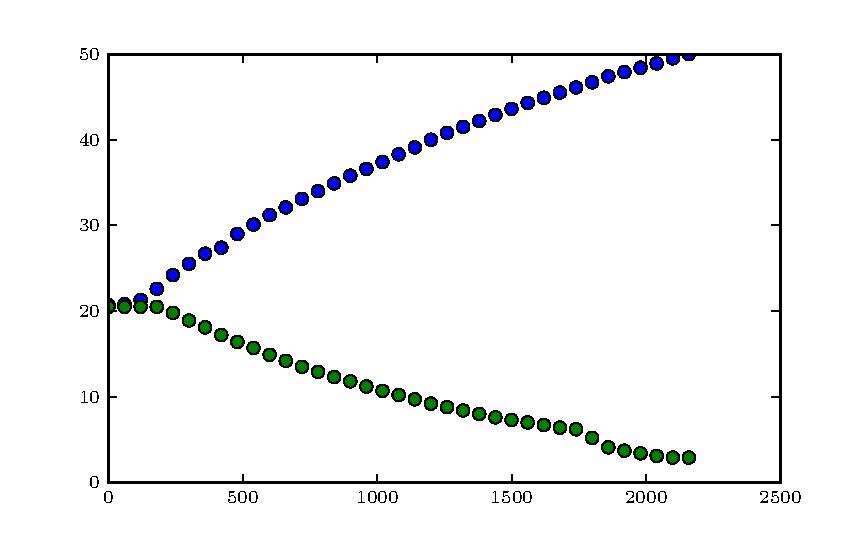
\includegraphics{plot.pdf}
%  \caption{Plot.}
%  \label{fig:plot}
%\end{figure}


%Tabelle
%\begin{table}
%	\centering
%	\caption{Table.}
%	\label{tab:table}
%	\begin{tabular}{ccc}
%		\toprule
%    column1&column2&column3\\
%		\midrule
%		220 & -391 & 659 \\
%		330 & -598 & 946 \\
%		525 & -1000 & 1660 \\
%		702 & -1337 & 2051 \\
%		930 & -1650 & 2450 \\
%		\bottomrule
%	\end{tabular}
%\end{table}
